
\section{Advances on cartographic document formats}\label{advances-on-cartographic-document-format}

The focus of this work is the definition of a novel format of cartographic
documents along with the software ecosystem rooted on it. A simple but
effective algorithm to find indoor valid routes is also provided. The
\textbf{HIJSON} (\textbf{H}ierarchical \textbf{I}ndoor \textbf{JSON}, this is
the name chosen for the format) and the accompanying software framework aim
to realize a mapping of indoor real spaces with a virtual interactive web
environment. The HIJSON is based upon ideas and design principles collected
from previous formats and identifies three critical improvements with respect
to them: it exposes a \emph{hierarchical structure}, uses \emph{metric local
coordinate system} and accepts \emph{semantic extensions}. Furthermore, geometrical 
and topological data are conveniently imported and represented via LAR, an advanced 
representation scheme, allowing to deal with \emph{hyperlinked geometric models}.

\subsection{Hierarchical structure}\label{hierarchical-structure}

The HIJSON format allows for hierarchical description of indoor spaces. The
introduction of a hierarchical structure establishes a parent-child relation
between entities of the model, reflecting a container-contained relationship.
This direclty implies a neater representation than the plain linear structure
adopted by GeoJSON, being a perfect analogy of objects contained (i.e.
placed) into spaces.

In addition, more organized arrangement is allowed by logical (or even
physical) grouping: concepts like building wings, sections, stories,
departemens, etc. can be introduced to reflect into the document structure
logical or physical real divisions, categories or relashionships.

Hierarchical structures are common in computer graphics since they are used as
scenegraphs. This accordance of underlying structures really simplify 3D
render algorithms of HIJSON documented environments.

Furthermore the container-contained relation enables to use local reference system.


\subsection{Hyperlinked geometric models}\label{optional-lar}

A HIJSON document may further import external geometric models---either of the buildings itself or the interior furniture or devices---that are topologically complete (in the sense of solid modeling~\cite{Requicha:1980:RRS:356827.356833}) and very compact. 
Such models coming from a source outside the document are acquired by linking JSON files that contain a Linear Algebraic Representation (LAR) of topology and geometry, to be expanded for visualization or interaction at any useful level of detail. 

The LAR scheme~\cite{Dicarlo:2014:TNL:2543138.2543294} is characterised by a very large domain, including architecture, building and construction~\cite{paoluzziMS:2014}, 2D and 3D engineering meshes, non-manifold geometric and solid models and meshes, and high-resolution 3D images~\cite{cadanda:2015}. This scheme uses the set of \emph{Combinatorial Cellular Complexes} (CCC) as mathematical domain
\cite{Basak:2010}, and various compressed representations of \emph{sparse matrices} \cite{gemmexp} as codomain. 

Since LAR provides a complete representation of the topology of the represented space,
the matrix $[\partial_d]$ of the boundary operator shall be used to compute the coordinate representation $[c]$ of the \emph{boundary} chain of \emph{any subset} $c$ of cells, though \emph{a single} operation of SpMV multiplication \cite{gemmexp} between the \texttt{CSR} (Compressed Sparse Row) representation of $[\partial]$ and the \texttt{CSC} (Compressed Sparse Column) representation of the $[c]$ chain, resulting in very efficient computations on modern hardware, even mobile.


% \begin{figure*}[htbp] % figure placement: here, top, bottom, or page
%  \centering
%  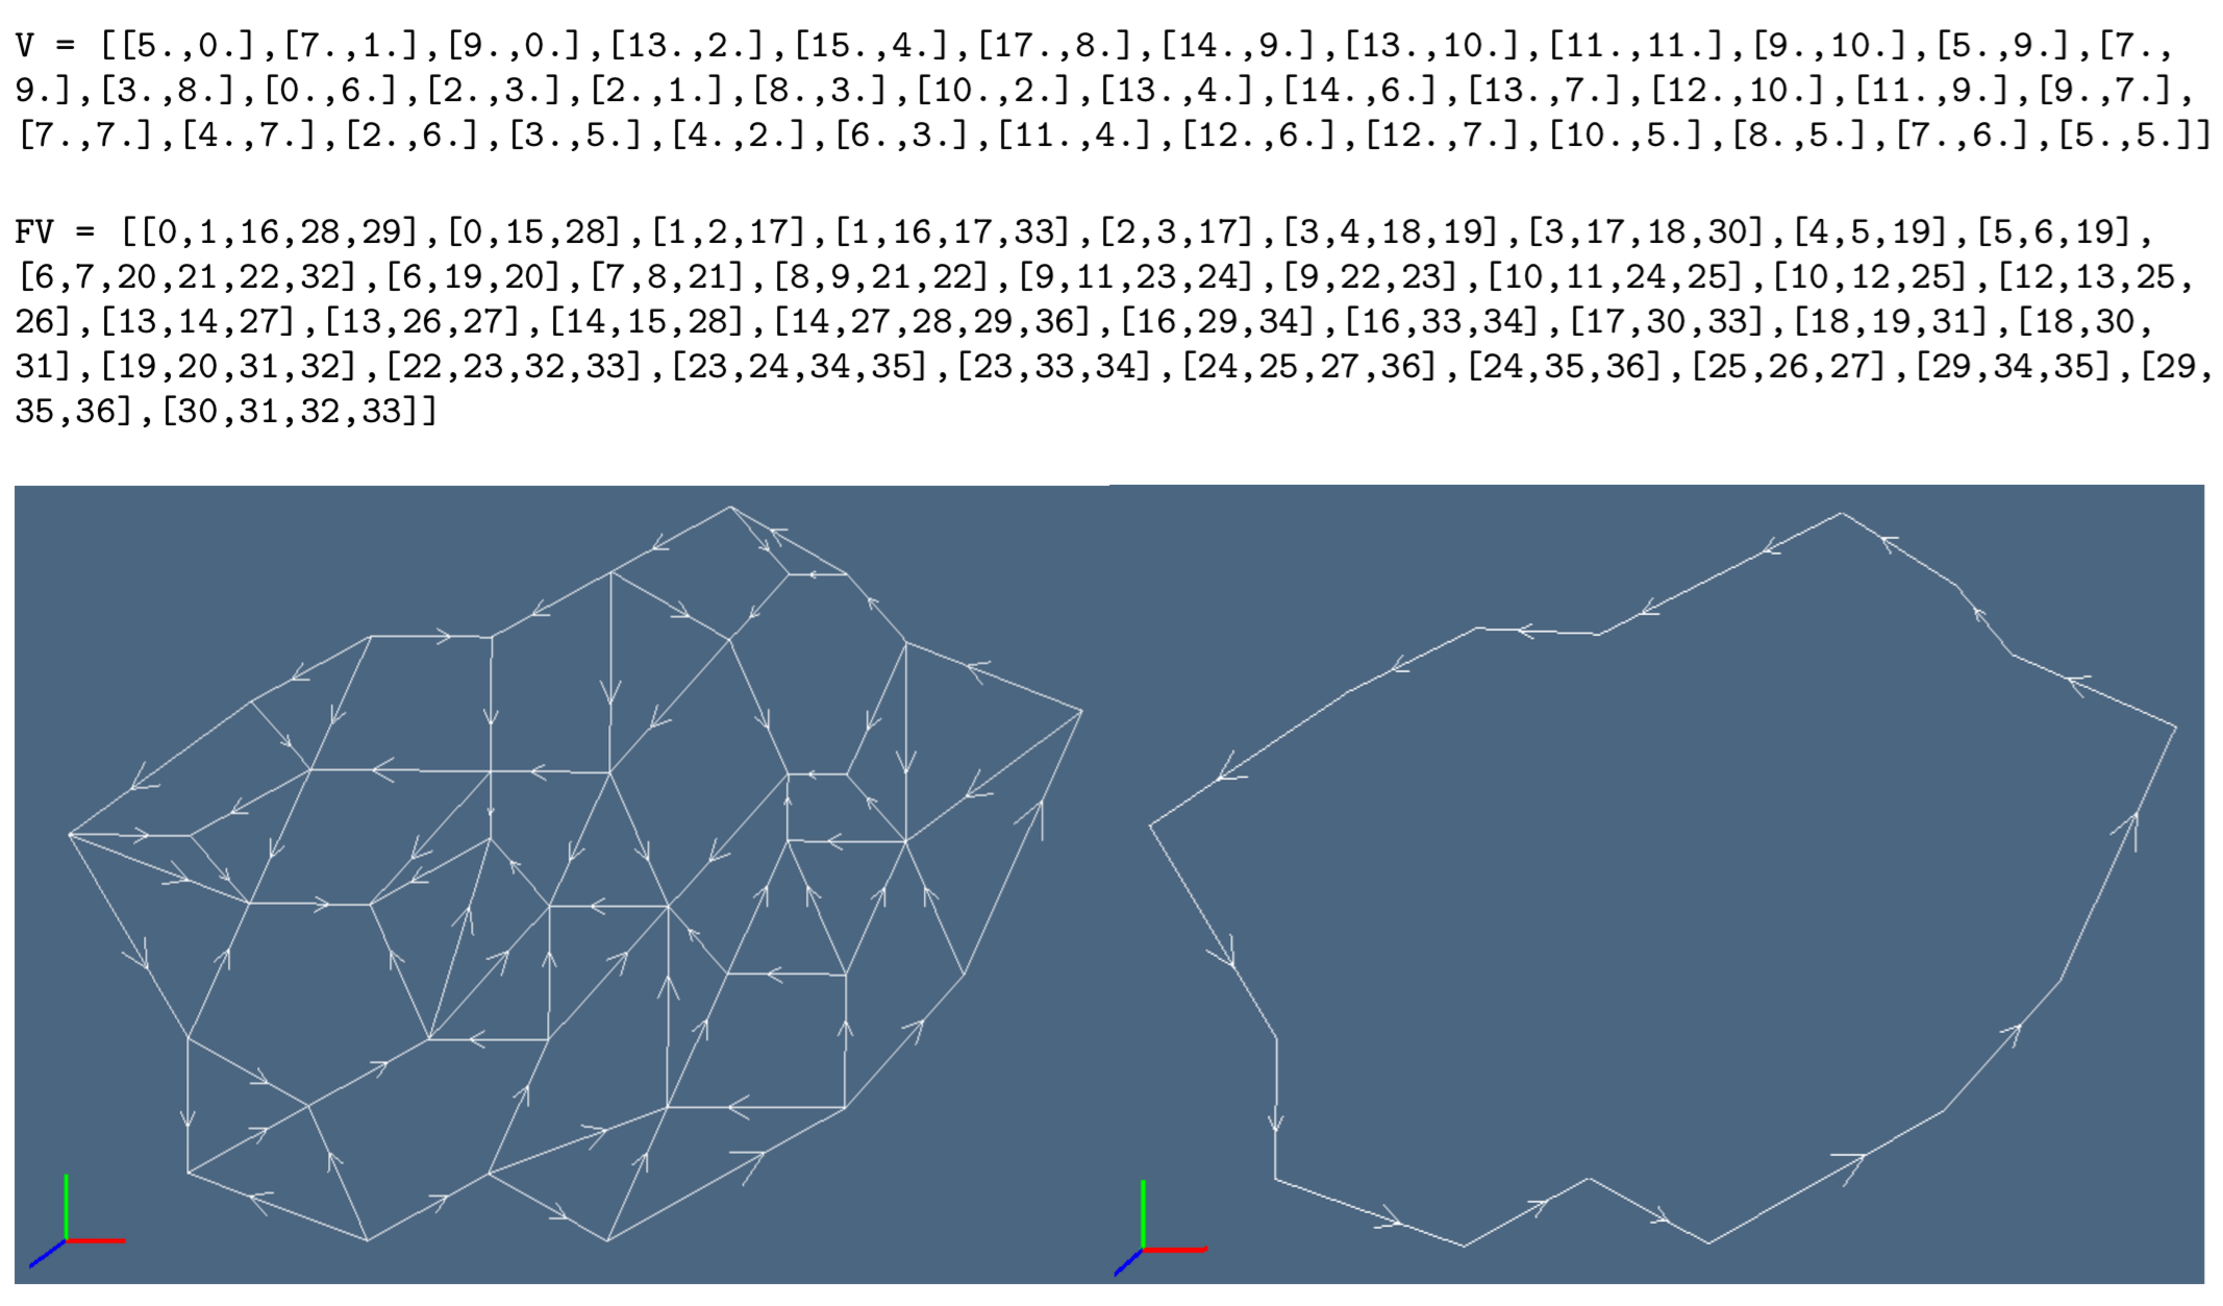
\includegraphics[width=0.5\linewidth]{images/minimum} 
%  \hfill
%  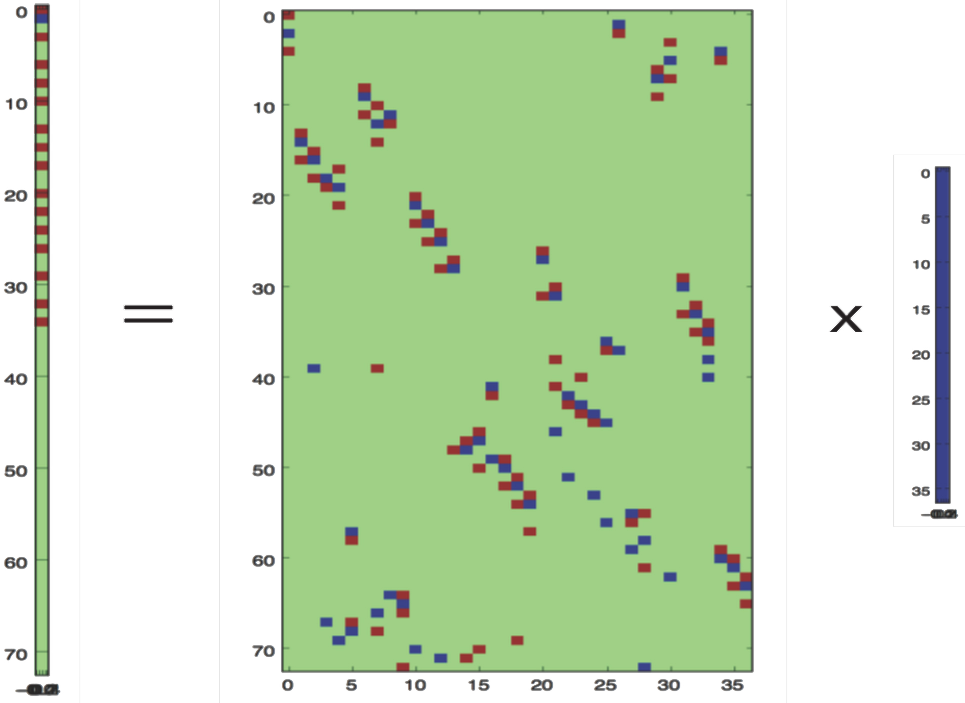
\includegraphics[width=0.4\linewidth]{images/boundary} 
%  \caption{A toy example of the LAR scheme: (a) the bare minimum of data with \emph{complete} information about topology; (b) the extracted boundary; (c) the extraction method $[e] = [\partial][f]$ giving the coordinate representation (in the discrete basis of the 1-cells) ofthe boundary edges $[e]$ by product of the sparse boundary operator matrix $[\partial]$ times the coordinate representation $[f]$ of the 2-cells (faces), in the discrete basis of the 2-cells.}
%  \label{fig:minimum}
% \end{figure*}


\begin{figure}[!h]
 \centering
 \begin{subfigure}[b]{\linewidth}
 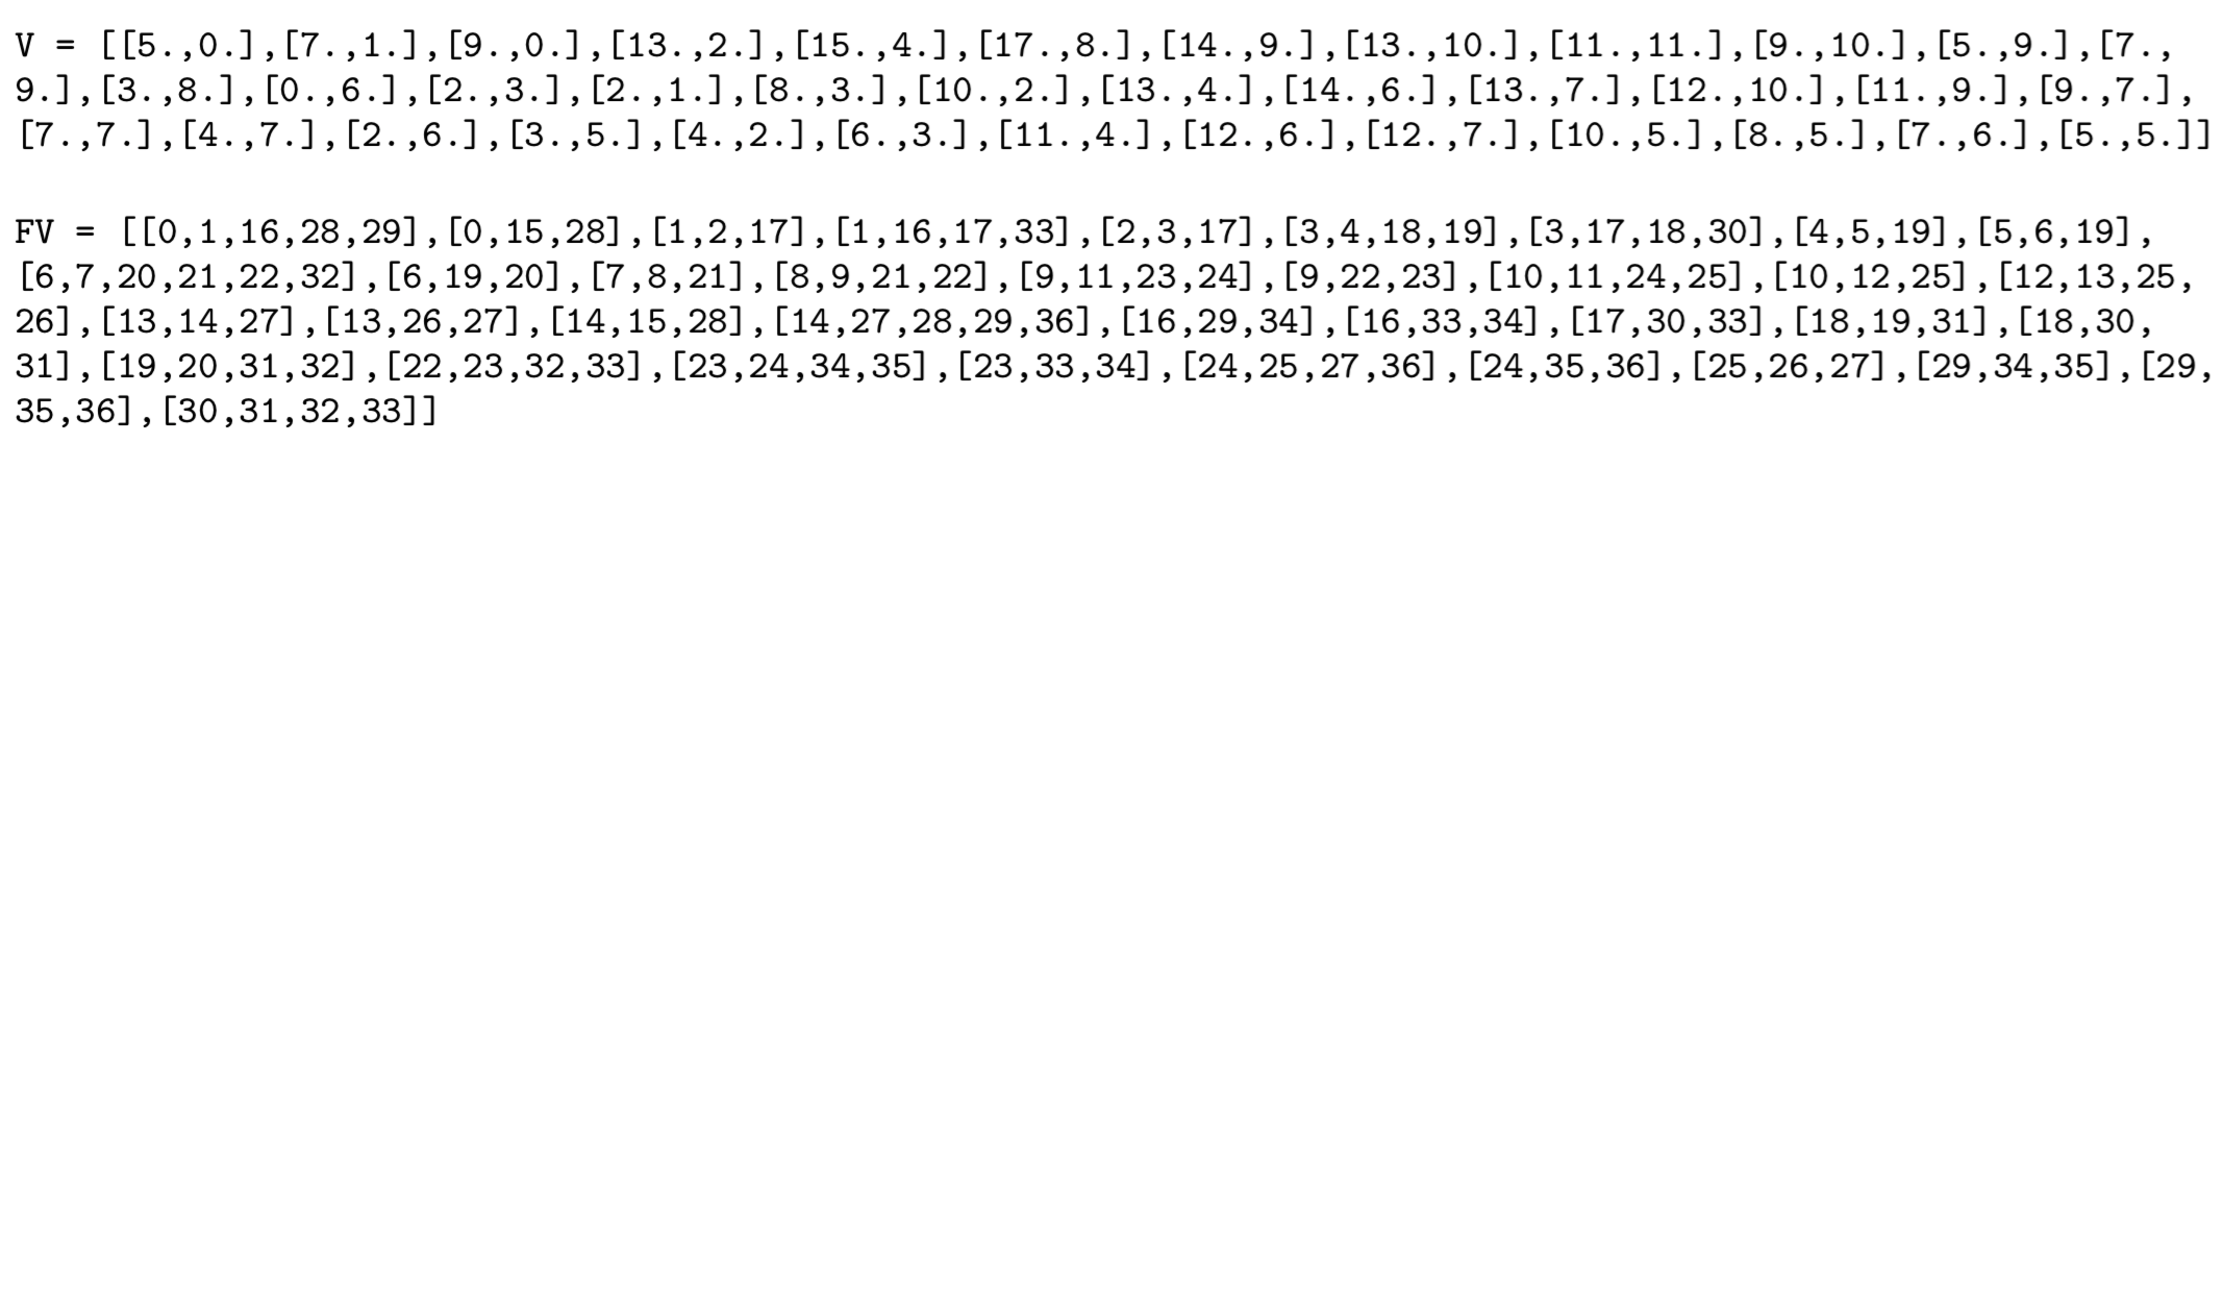
\includegraphics[width=\textwidth]{images/minimum-data}
 \end{subfigure}
\\
 \begin{subfigure}[b]{0.48\linewidth}
 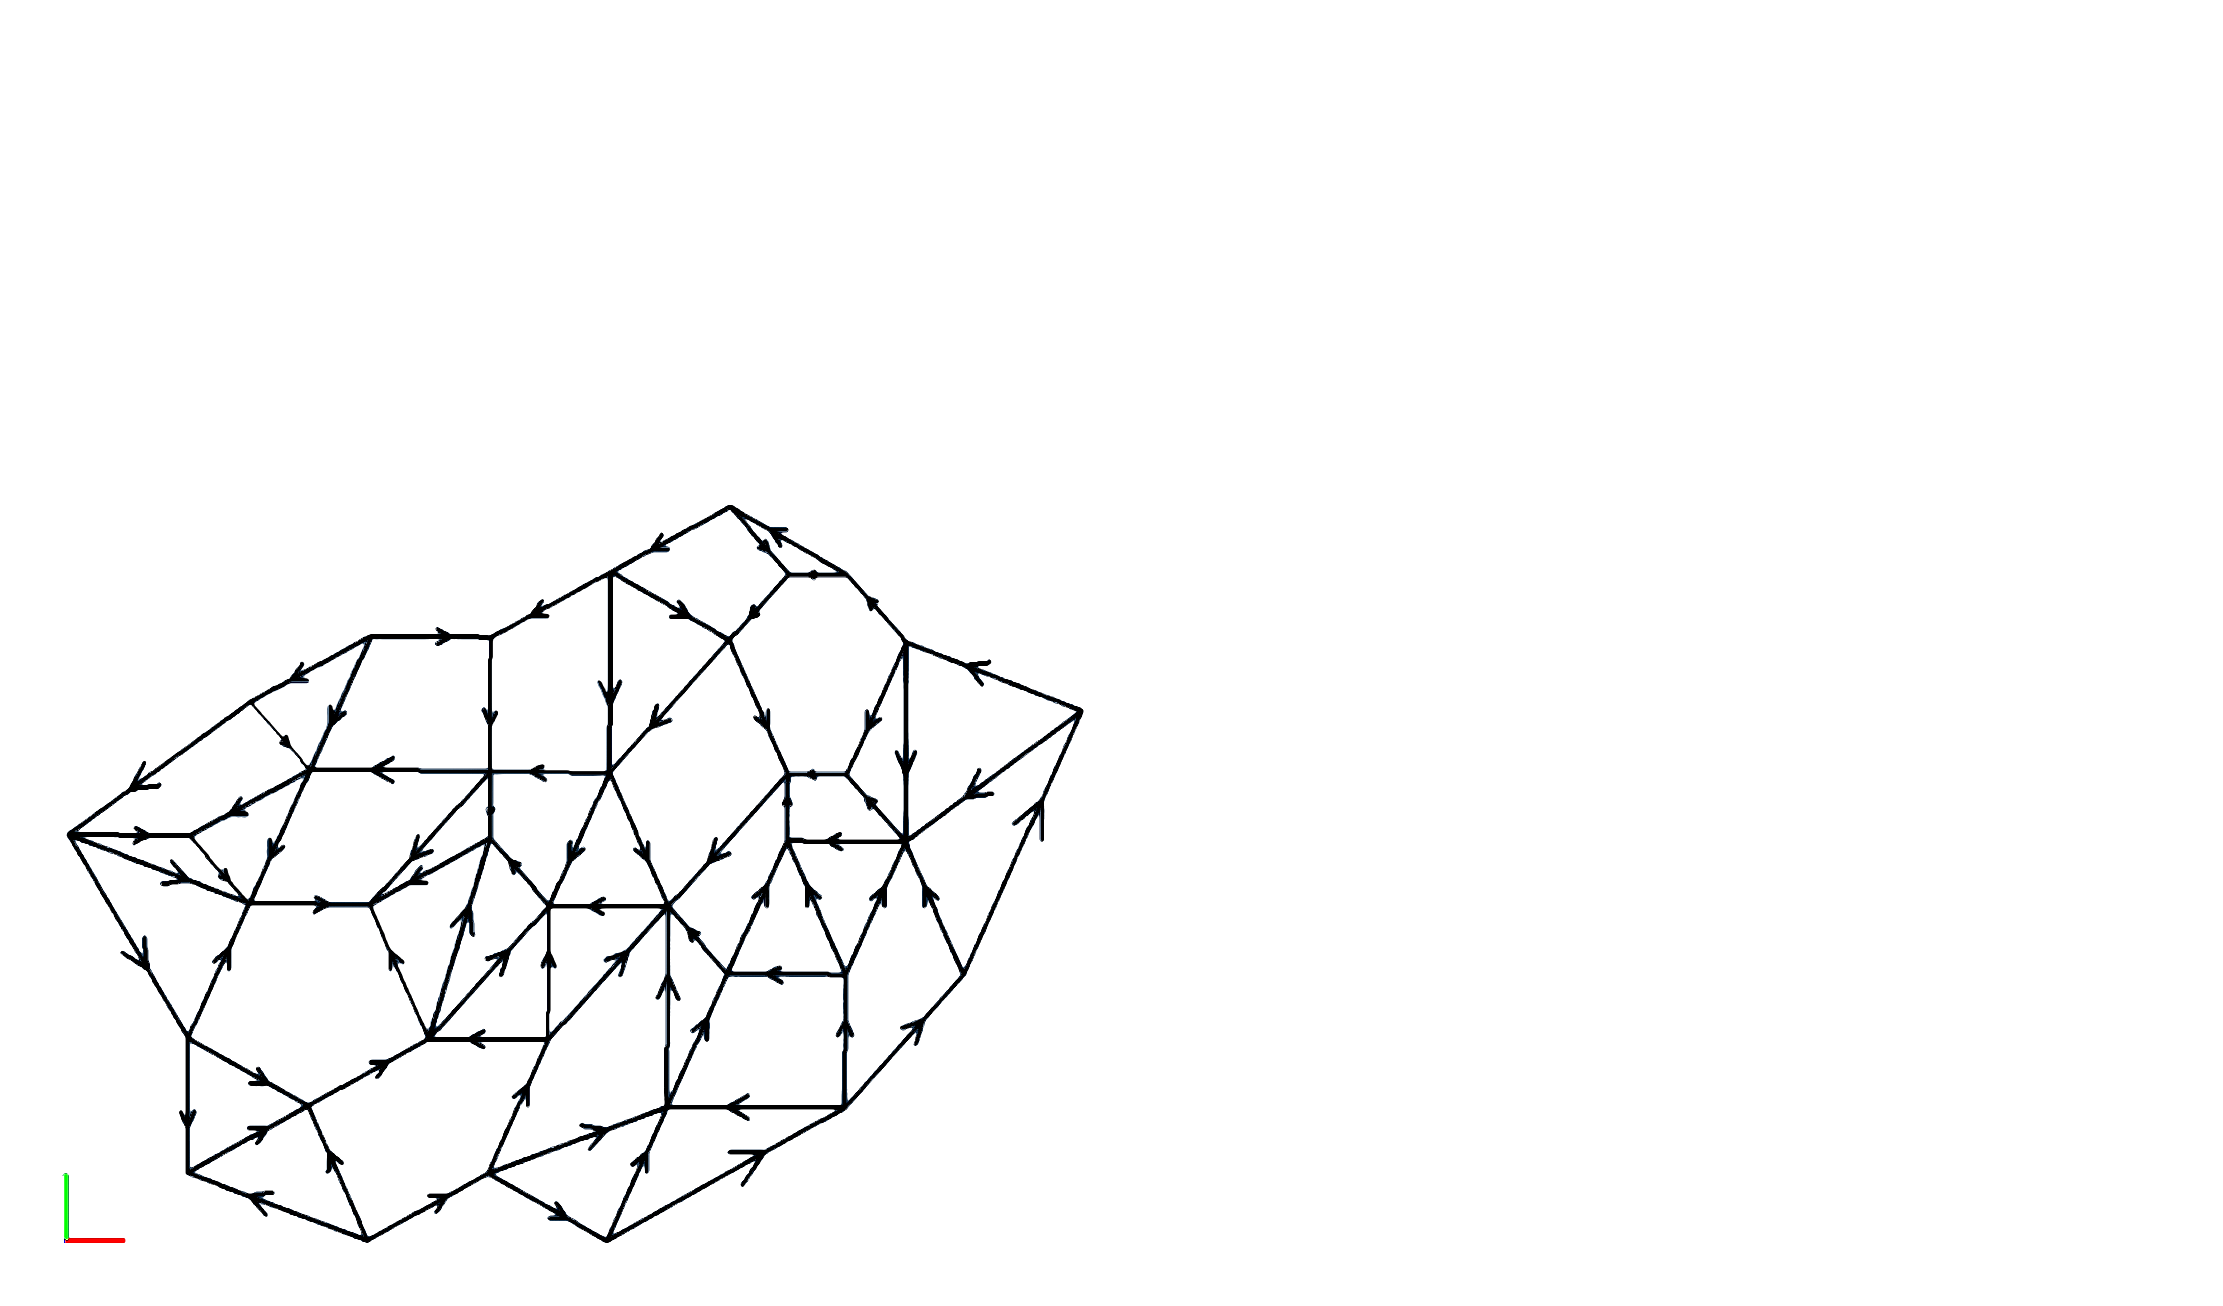
\includegraphics[width=\textwidth]{images/minimum-colors-a}
 \caption{}
 \vspace*{4mm}
 \end{subfigure}
 ~
 \begin{subfigure}[b]{0.48\linewidth}
 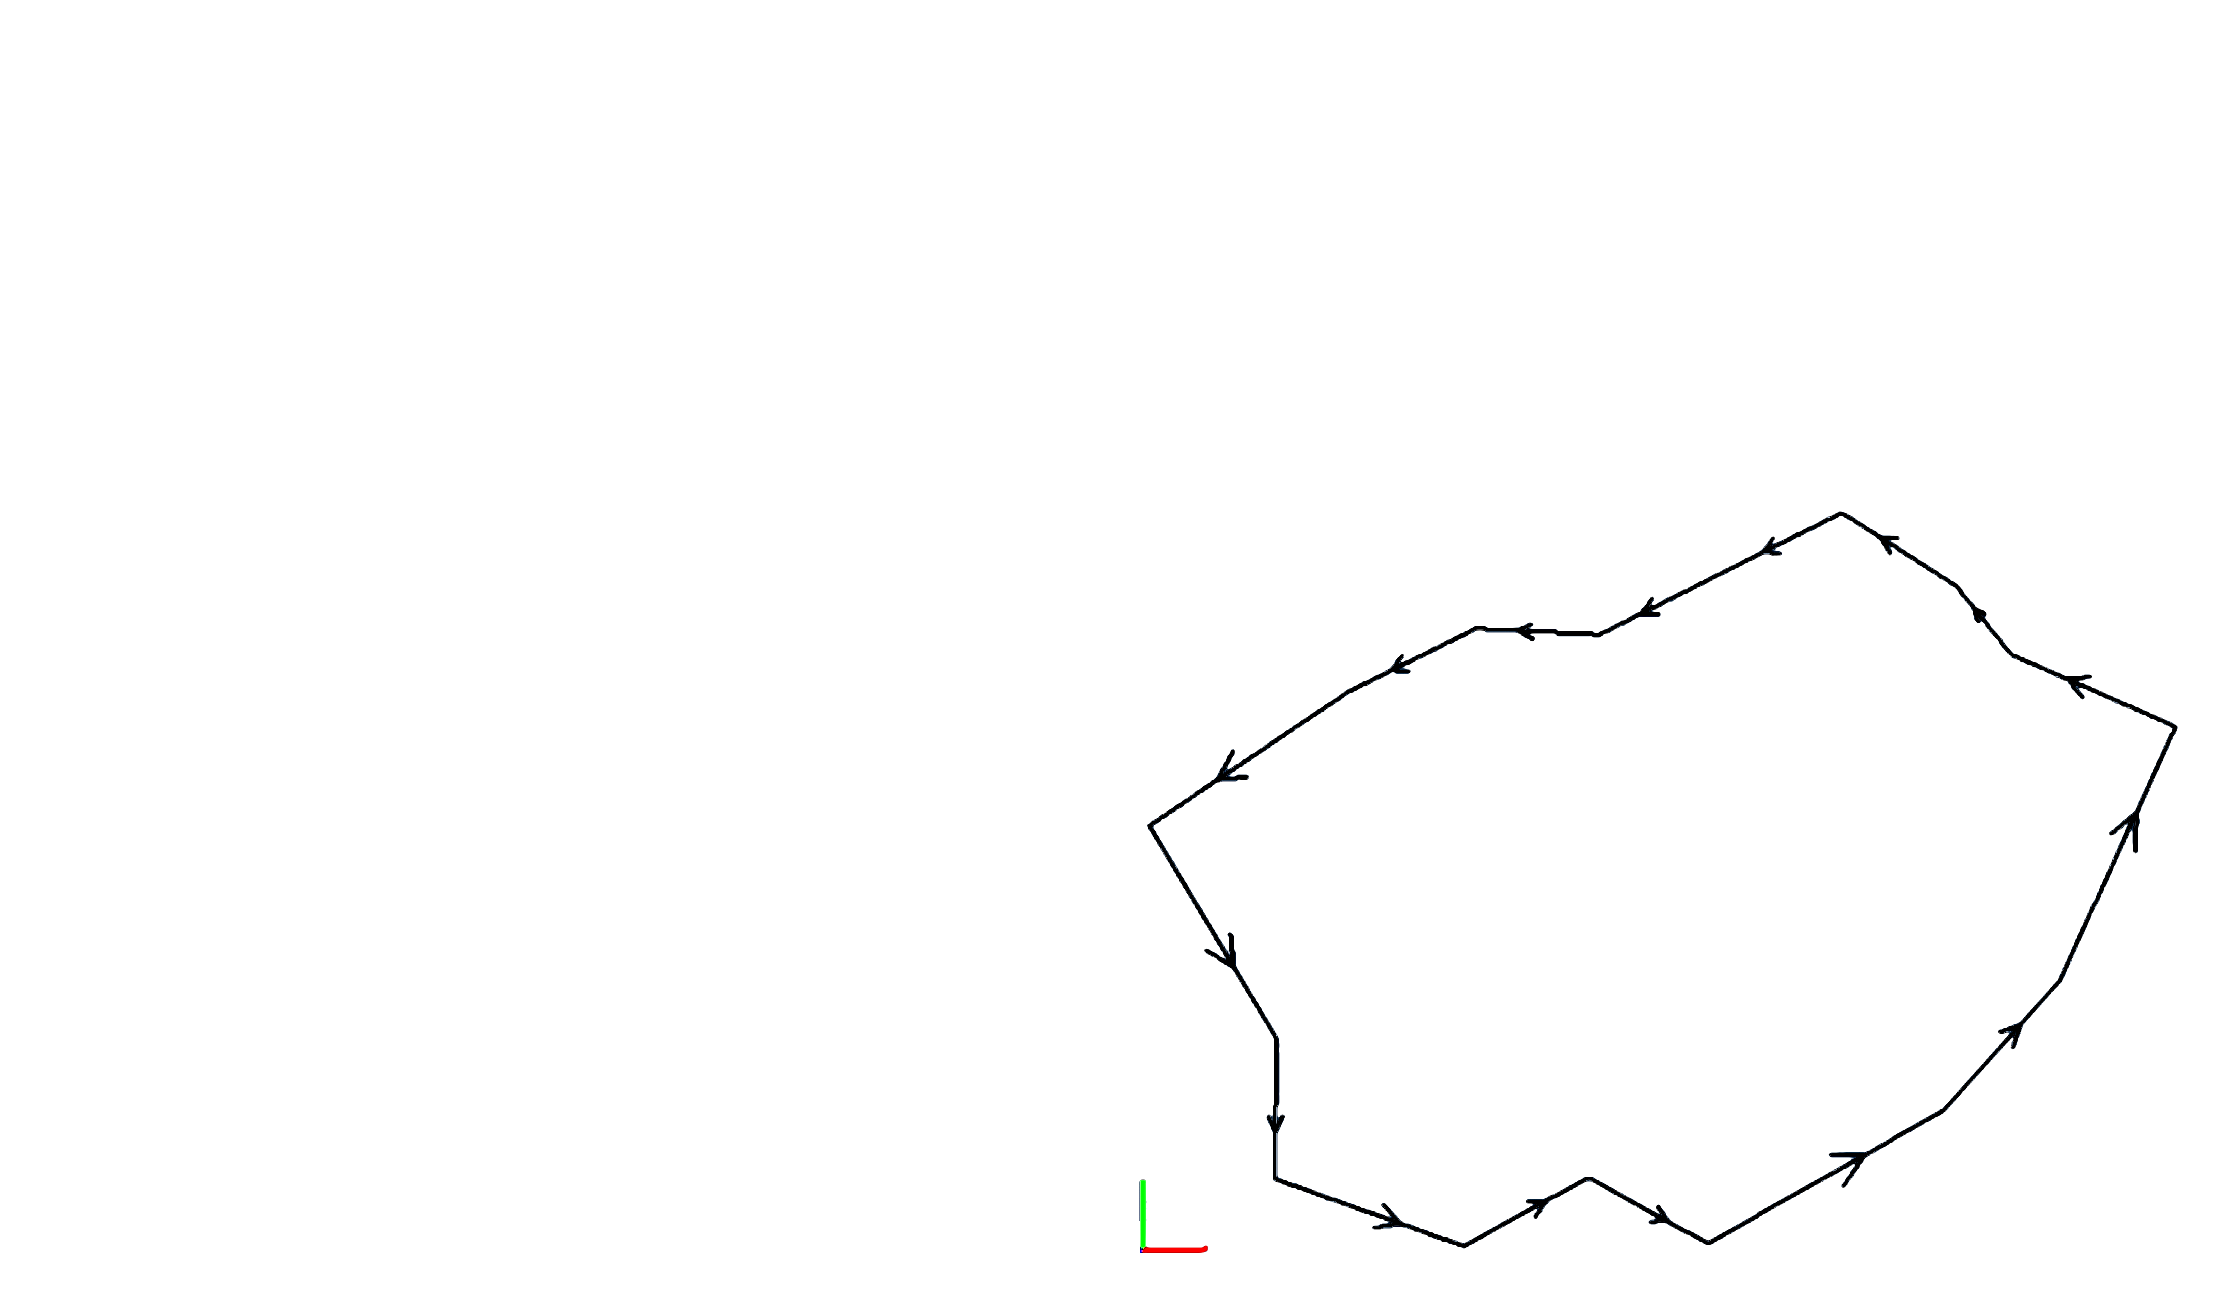
\includegraphics[width=\textwidth]{images/minimum-colors-b}
 \caption{}
 \vspace*{4mm}
 \end{subfigure}
\\
 \begin{subfigure}[b]{0.6\linewidth}
 \centering
 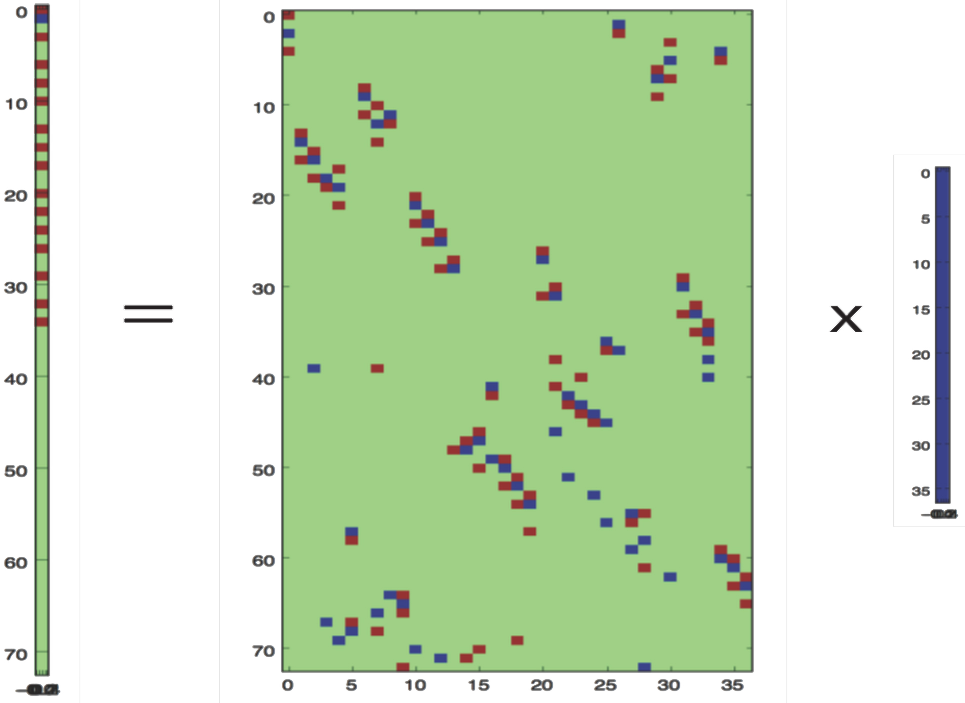
\includegraphics[width=\textwidth]{images/boundary}
 \caption{}
 \end{subfigure}
 
 \caption{A toy example of the LAR scheme: (a) the bare minimum of data with \emph{complete} information about topology; (b) the extracted boundary; (c) the extraction method $[e] = [\partial][f]$ giving the coordinate representation (in the discrete basis of the 1-cells) ofthe boundary edges $[e]$ by product of the sparse boundary operator matrix $[\partial]$ times the coordinate representation $[f]$ of the 2-cells (faces), in the discrete basis of the 2-cells.}
 \label{fig:minimum-data}
\end{figure}



The expansion of a LAR model, to be considered as a general-purpose graphic primitive, may be executed on either the server or the supervisor client of the HIJSON Web Toolkit architecture (see Section~\ref{server-architecture}), or even on the explorer client, depending on the size and the locality of the model to be expanded.

% \begin{figure}[htbp] % figure placement: here, top, bottom, or page
% \centering
% \includegraphics[width=\linewidth]{images/sogei} 
% \caption{Office building: (a) the schematic plan; (b) the simplified 3D model generated for testing on the field the in-door mapping project described in this paper.}
% \label{fig:sogei}
% \end{figure}

\begin{figure}[!h]
 \centering
 \begin{subfigure}[b]{0.48\linewidth}
 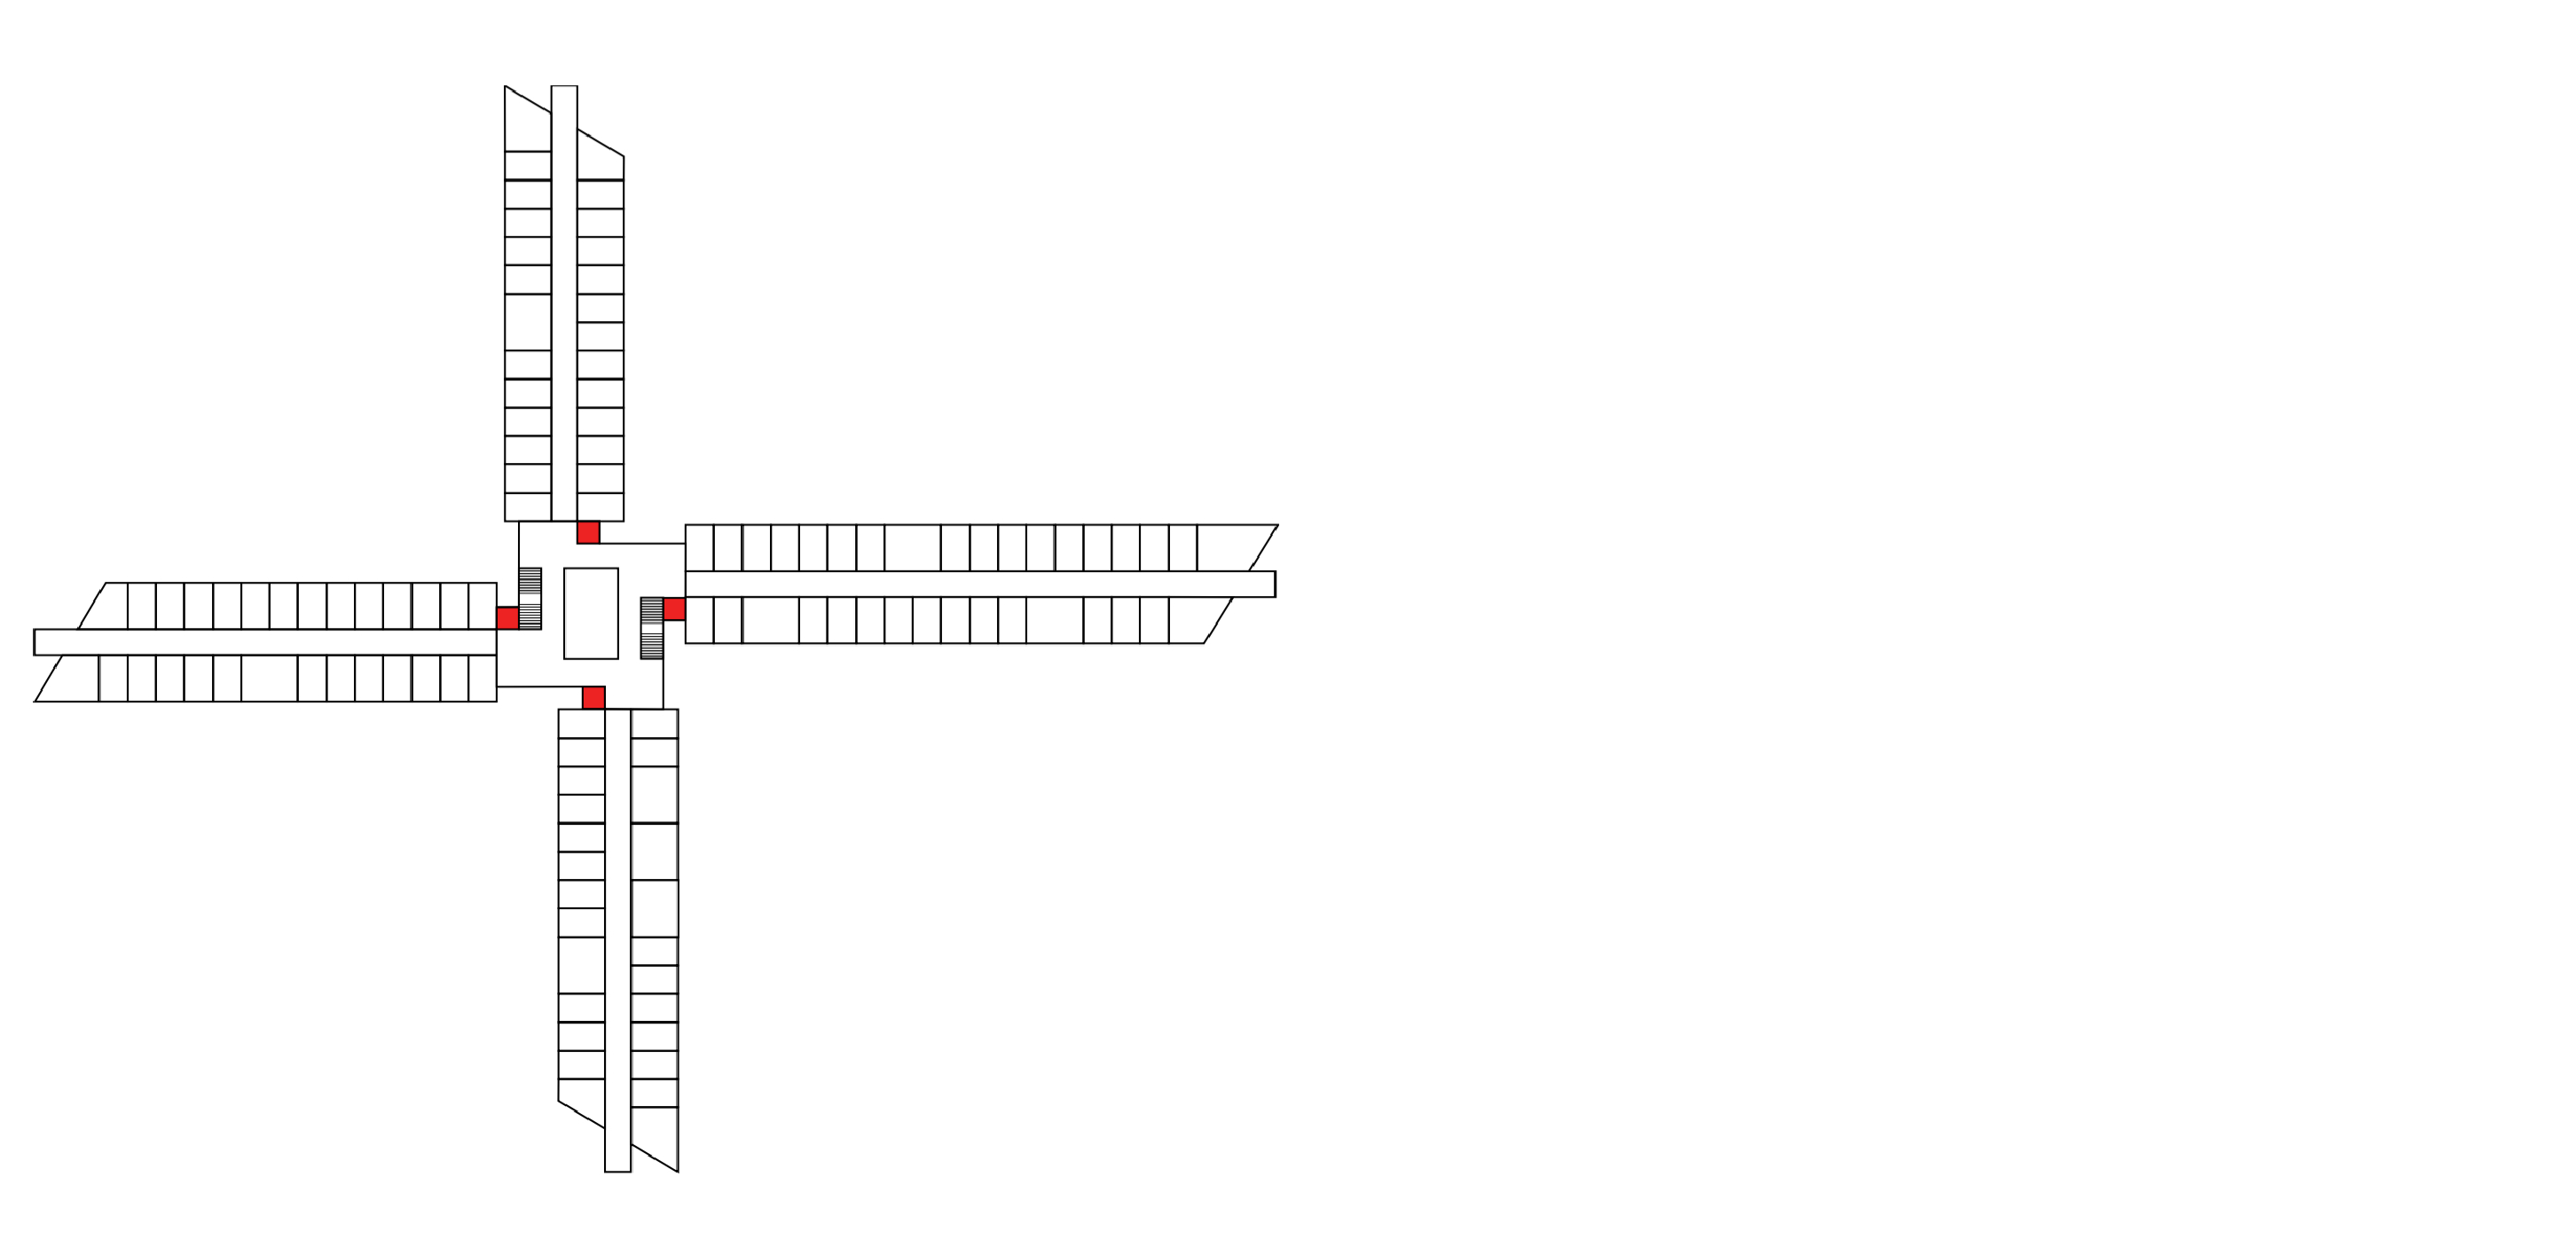
\includegraphics[width=\textwidth]{images/sogei-a} 
 \caption{}
 \label{fig:sogei-a}
 \end{subfigure}
 ~
 \begin{subfigure}[b]{0.48\linewidth}
 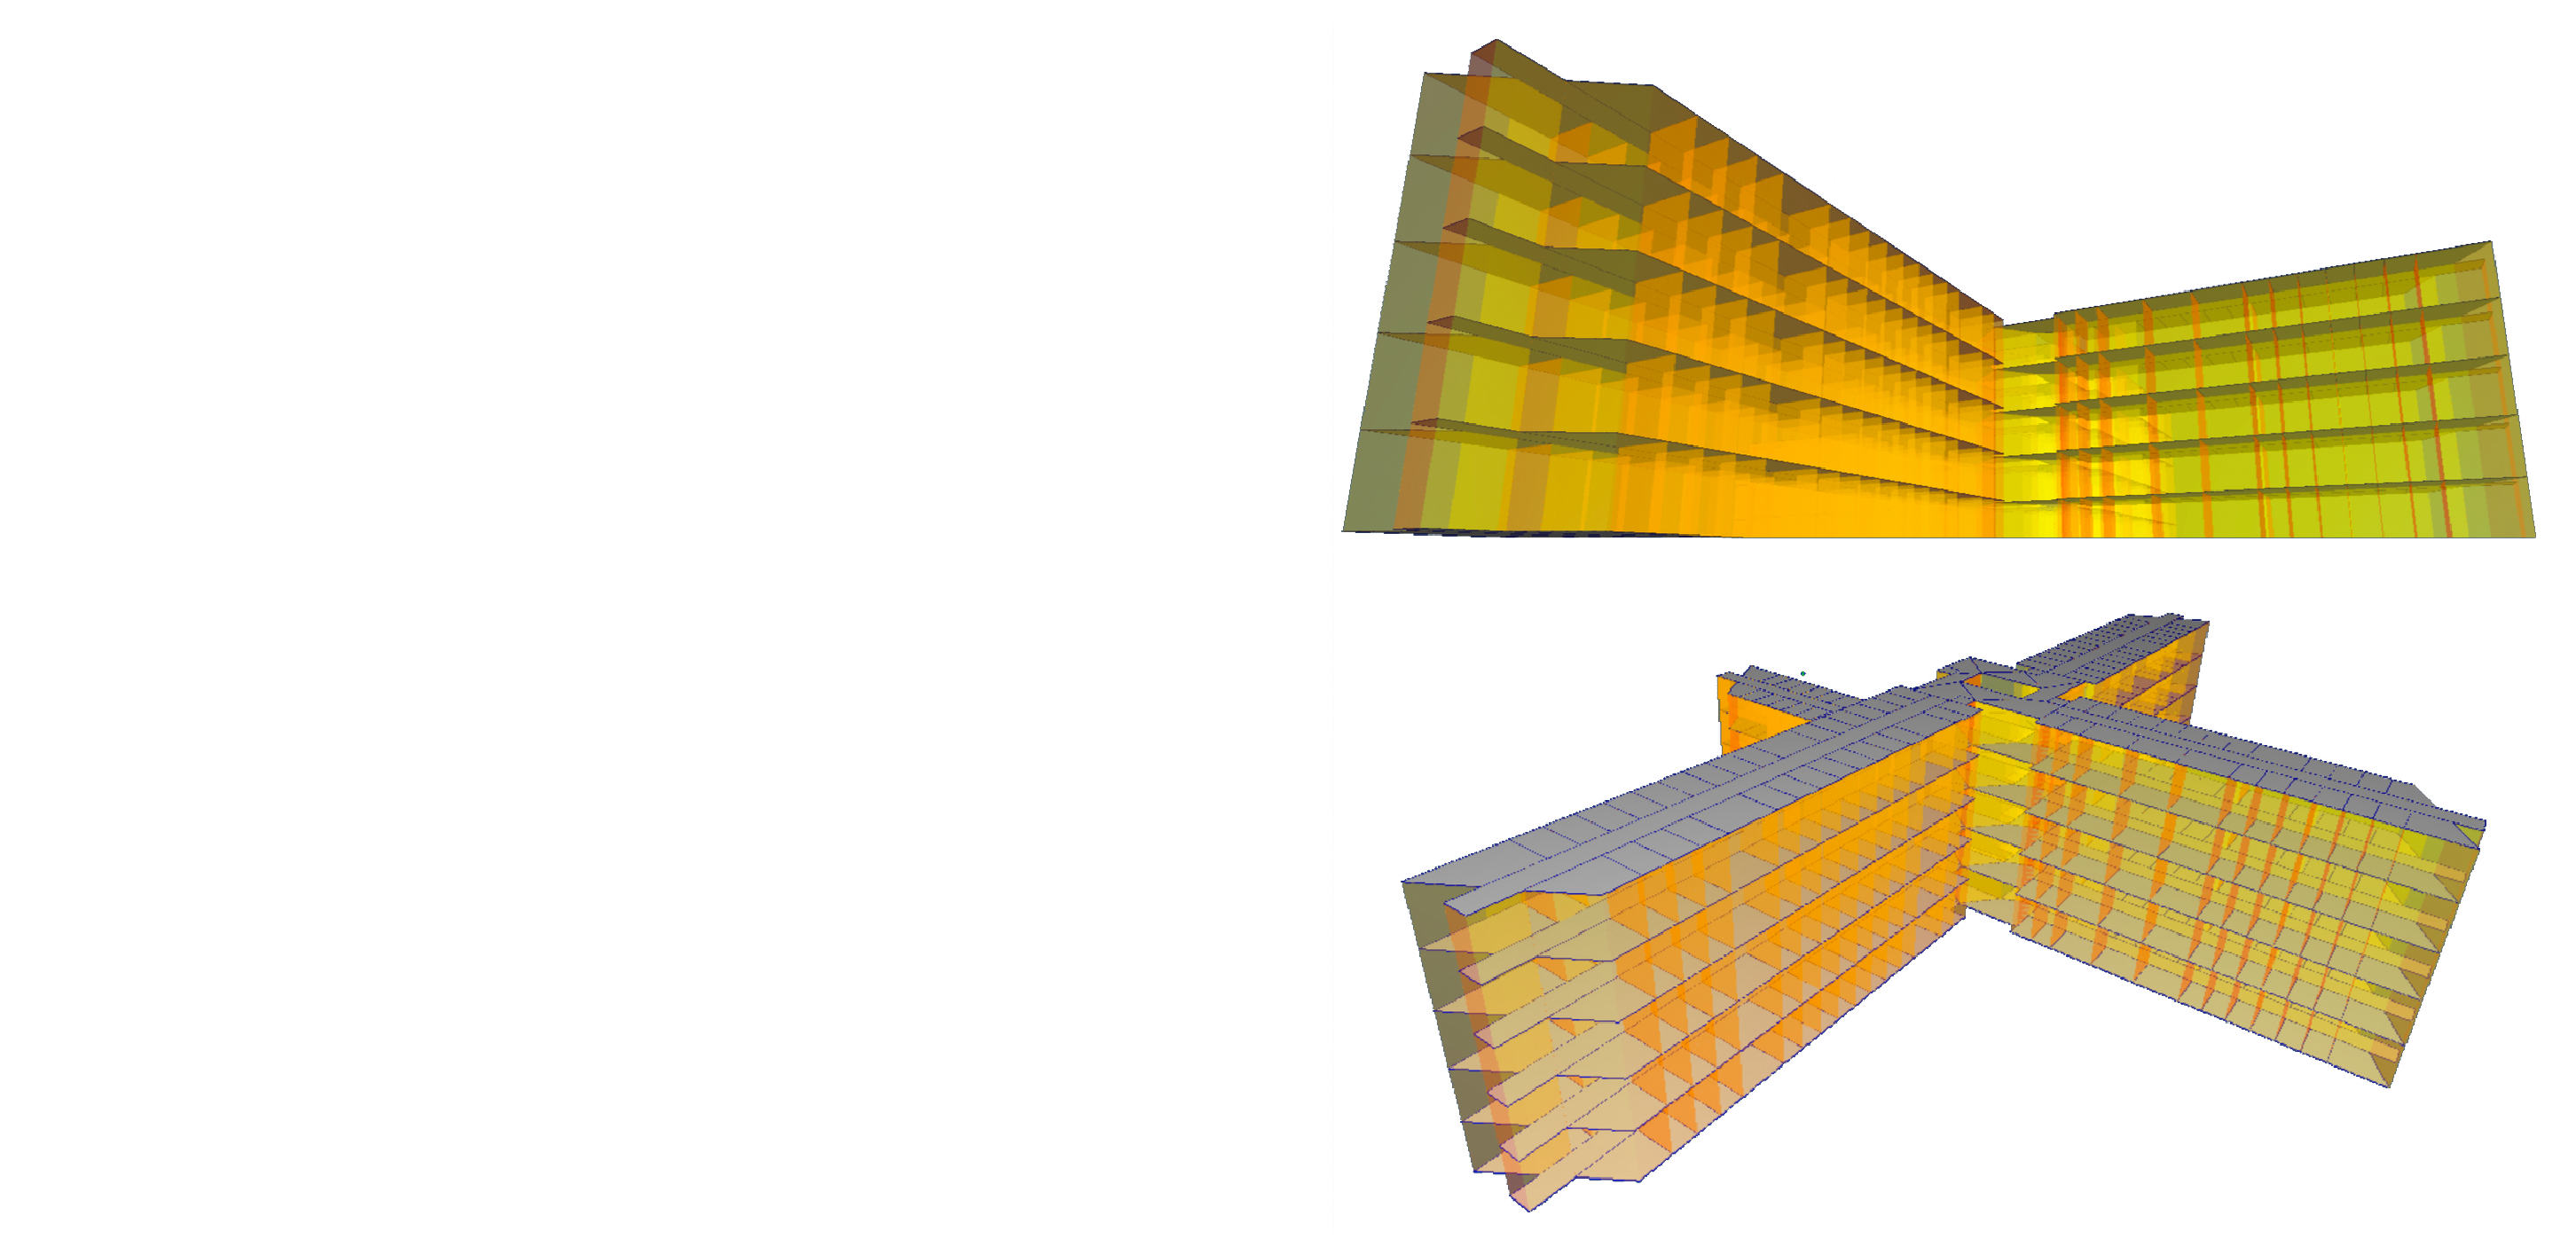
\includegraphics[width=\textwidth]{images/sogei-b}
 \caption{}
 \label{fig:sogei-b}
 \end{subfigure}
 
 \caption{Office building: 
 (a) the schematic plan; 
 (b) the simplified 3D model generated for testing on the field 
 the in-door mapping project described in this paper.
 }
 \label{fig:sogei}
\end{figure}

\subsection{Metric local coordinate system}\label{metric-local-coordinate-system}

Supported by the hierarchical underlying structure, the HJSON document format allows 
for the use of local coordinate system. This means that the shape of all elements can 
be convenient modelled in local coordinate and than placed in the right position 
with respect to the position of the parent (or container) element applying a 
translation and a rotaction vector.

Another substantial advantage is represented by the adoption of a metric reference, 
consequently simplifying the compilation of the document, however it is, 
manual or aided by software tools.

The HIJSON document format is specially designed to guarantee the user to be routed seamlessly 
from outdoor to indoor and vice versa. Even though indoor geometries are inputted in a metric 
local continuous outdoor-indoor navigation is ensured via the definition of a processing pipeline
detailed in the following.

\subsection{Semantic extensions}\label{semantic-extensions}

Semantic extensions make the HIJSON format extendible and customizable, that
is, able to adequately respond to any object representation need. To define a
semantic extension means to allow the HIJSON document to model an object
previously not covered, or even to modify the behaviour of a comprised one.
Semantic extensions are to be defined both as HIJSON format syntyax and as
HIJSON Toolk source code. In particular it is necessary to define respectively
a new HIJSON Element and a new HIJSON Class, as specified below.

